\section{Introduction And Motivation}
\subsection{Introduction To Blockchain}
\textit{“Blockchain is a continuously growing list of records, called blocks, which are linked and secured using cryptography. Each block contains typically a hash pointer as a link to a previous block, a timestamp and transaction data”} \cite{wiki:001}. It can serve as a distributed ledger that can record transactions without a central server or trusted third party. The transactions are available to all parties and are easily verifiable. It is inherently resistant to data tampering as altering data in any one block breaks the chain and requires that all subsequent blocks be calculated again using the new data. Technical details of blockchains are discussed in chapter \ref{Blockchain}, however for a high level overview please refer to figure \ref{fig:blockchain}. Notice that each block has a unique signature or hash and is linked to previous blocks through its hash. Blockchain has the power to revolutionize how business is conducted in the digital age. Some people are calling it the most important innovation since the development of the internet and the world wide web. The proponents of this technology believe that it will fundamentally transform the web itself. Internet of tomorrow will be powered by decentralized applications or Dapps \cite{misc:020}. The first blockchain was Bitcoin, it was invented by a person or group of persons known only by the pseudonym Satoshi Nakamoto. Bitcoin is a form of peer-to-peer electronic cash designed to transfer value between two parties without involving banks or other financial institutions. It was the first to solve the double spend problem without using a central server. Bitcoin paved the way for exponential growth in crypto currency market which together with other Altcoins is worth over 120 billion dollars at the time of writing. The underlying technology which powers Bitcoin, Ethereum and other crypto currencies can be used for much more than just transferring X amount of coins from Person A to Person B. Researchers are employing blockchain technologies to increase efficiency and reduce costs in industries such as Supply Chain Management, Internet of things, Banking and Finance to name a few.

\begin{figure}[b]
	\centering
    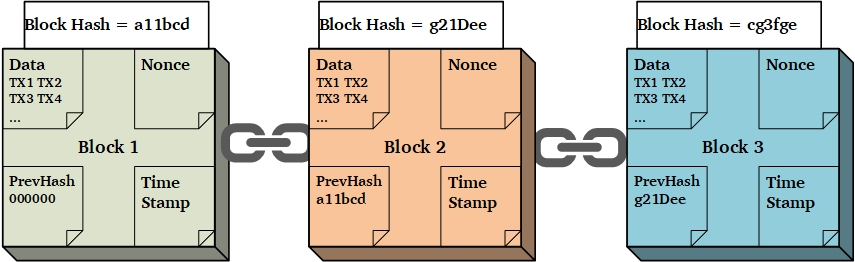
\includegraphics[width=160mm,scale=0.5]{figs/blockchain}
	\caption{High Level Overview of the Blockchain}
	\label{fig:blockchain}
\end{figure}
\clearpage  
\subsection{Blockchain Types}
Blockchain technologies have experienced rapid growth in the recent years. The rapid pace of innovation has given rise to new models, paradigms and technologies in this sector. We now have multiple competing blockchain networks and solutions jostling for different segments of the market. There is Monero and Zcash focusing on privacy oriented solutions employing technologies like ring signatures \cite{paper:008} and zk-SNARKS. Others like Ripple and Hyper Ledger are tailoring their solutions for specific segments of the market like banking and enterprise. This accelerated pace of innovation has ignited a fierce debate in the community as to what can and cannot be classified as a blockchain. The classification schemes consider range of different factors,  including design and architecture of the underlying blockchain protocol. In the paper presented in \cite{7930224} the authors classify blockchain systems based on their architecture and the level of decentralization i.e. Fully Centralized, Partially Decentralized, and Fully Decentralized. Most publications and experts however, classify blockchains into two broad categories: Public or Permissionless Blockchains, and Private or Permissioned Blockchains \cite{misc:017}. This classification is useful as it uses a range of functional and non-functional properties of blockchain systems for categorizing them.
%\bigskip
\vspace{1cm}
\begin{table}[h]
\begin{tabular}{|l|l|l|}
\hline
                          & \multicolumn{1}{c|}{\textbf{Permissionless Blockchains (Public)}} & \multicolumn{1}{c|}{\textbf{Permissioned Blockchains (Private)}} \\ \hline
\textbf{Network Access}   & Any one can join the network                                      & Only authorized participants can join                            \\ \hline
\textbf{Minning}          & Any one can produce new blocks                                    & Authorized block producers                                       \\ \hline
\textbf{Decentralization} & Fully decentralized system                                        & Can have limited to no decentralization                          \\ \hline
\textbf{Speed}            & Slower compared to private blockchains                            & Faster                                                           \\ \hline
\textbf{Transparency}     & Fully transaparent                                                & Customizable level of transparency                               \\ \hline
\end{tabular}
\caption {Permissioned vs Permissionless Blockchains}
\end{table}
%\clearpage  
\vspace{1cm}
\subsubsection{Permissionless Blockchains} 
Permissionless or Public blockchains are highly decentralized networks that value decentralization and censorship resistance above everything else. Permissionless systems allow any person or entity to interact with the network or run smart contracts \cite{arXiv:1806.03693}. Every participant has equal rights to create, send, and view transactions. They can even choose to become block producers or miners and verify transactions in order to append them to the blockchain. 

Bitcoin was the first public blockchain and a realization of a vision outlined by Satoshi in his white paper \cite{paper:001}. He identified decentralization, censorship resistance and distributed trust as the most important factors for the success of the peer-to-peer digital cash protocol he proposed. The main functional and non-functional properties of permissionless systems are given below:
\clearpage
\textbf{Decentralization:}
Public blockchains are usually highly distributed and decentralized. This makes the network censorship resistant and harder to attack and bring down by any one entity. 

\textbf{Consensus Mechanisms:}
Decentralization is achieved at the cost of higher complexity hence public blockchains requires sophisticate consensus mechanisms. There are two main types of consensus mechanisms: Proof of Work [\ref{PW}], and Proof of Stake [\ref{PS}]. Any participating node can run the consensus software in order to verify transactions and extend the blockchain \cite{arXiv:1806.03693}, \cite{misc:017}.

\textbf{Block Producers:}
Any node can choose to become a block producer or miner. Public blockchains usually employ a crypto economic model where by miners are rewarded using network assets or tokens \cite{paper:001}.

\textbf{Privacy:}
Without a central entity or coordinator, transparency becomes an important feature for the participants and miners for establishing trust in the system. This transparency is often achieved by sacrificing some degree of privacy. By default, all transactions and data in a blockchain is public and can be easily accessed with the help of a block explorer.  
\vspace{1cm}
\subsubsection{Permissioned Blockchains}
Permissioned blockchains are sometimes also referred to as private blockchains. It is a closed ecosystem where participants need permission from an administrator or special node to interact with the ledger. Only pre-approved nodes or block producers can verify transactions and run smart contracts \cite{arXiv:1806.03693}. Participants place some level of trust in these block validators or administrators. 

Permissioned blockchains can be managed by members of a consortium in order to increase transparency and efficiency of inter organizational processes. They allow organizations to have better control over proprietary data while facilitating trusted exchange of secure information across organizational hierarchy \cite{arXiv:1806.03693}, \cite{misc:017}. The main functional and non-functional properties of permissioned blockchain systems are given below: 

\textbf{Decentralization:}
Permissioned systems can have varying degrees of decentralization. They can be fully centralized or partially decentralized. Systems like Hyperledger fabric allow fine grained control over governance models and the level of decentralization. The level of decentralization in permissioned systems depends upon many factors including number of participants, their relationship with each other, degree of required fault tolerance, business rules and consensus algorithms \cite{arXiv:1806.03693}, \cite{misc:017}.
\clearpage
\textbf{Consensus Mechanisms:}
Permissioned blockchains usually do not need to run complex consensus algorithms. They can run simplified consensus mechanisms. This coupled with the fact that only a limited number of nodes are responsible for producing new blocks helps them become more efficient and scalable \cite{arXiv:1806.03693}, \cite{misc:017}. 

\textbf{Block Producers:}
Private blockchains can set out criteria for participants to become block producers. These criteria can be based on certain business rules or participating nodes might be required to meet special conditions in order to become block producers such as demonstrating certain capabilities like minimum hash power, or having possession of certain assets etc. Unlike public blockchains block producers are not rewarded with network assets rather they work together to increase efficiency, reduce business costs and boost productivity \cite{arXiv:1806.03693}, \cite{misc:017}.
   
\textbf{Privacy:}
They can offer fine grained control over transaction visibility as opposed to public blockchains where basically any one can view any transaction by simply querying the blockchain or using a block explorer. This is a huge incentive for organizations to use permissioned blockchains as they might wish to prevent unauthorized disclosure of sensitive information \cite{arXiv:1806.03693}, \cite{misc:017}.
\clearpage
%\vspace{1cm}
\subsection{Motivation}
Blockchain has exploded as the technology of the future for several industries including cross border payments, peer to peer transactions, regulatory compliance, healthcare and supply chain management \cite{misc:021}. It provides a tamper proof immutable ledger which can be particularly useful in tracking goods and services as they move and change hands across borders in the supply chain. It enables new and innovative means of organizing and tracking data. In the modern era industries are highly interconnected through complex supply chains with their partners and suppliers across the globe. The success of a supply chain depends upon the integration and coordination of all of its participants. Figure \ref{fig:Airbus} shows the example of an Airbus A380. It is made up of four million individual parts and is built in six different sections in plants around Europe. Its wings are manufactured in Wales, the fuselage comes from Hamburg, Germany and the final assembly takes place in Toulouse. This cross border and federated model of manufacturing is possible only through Just-in-time (JIT) manufacturing and supply chains. Airbus and other multinational companies depend on JIT to ensure that their products and services are competitive in the global market. JIT processes depend upon sophisticated supply chain management and inventory tracking systems to maximize cost-efficiency and minimize delays. Transparency, efficient communication and quick dispute resolution are key to the success of any supply chain. Traditional supply chain management systems are mostly centralized and siloed inside organizational structures. These systems are highly dependent on human actors to update the state of the system. This can lead to side effects such as increased complexity, reduced efficiency, and human errors.
%\clearpage 

\begin{figure}[h]
	\centering
    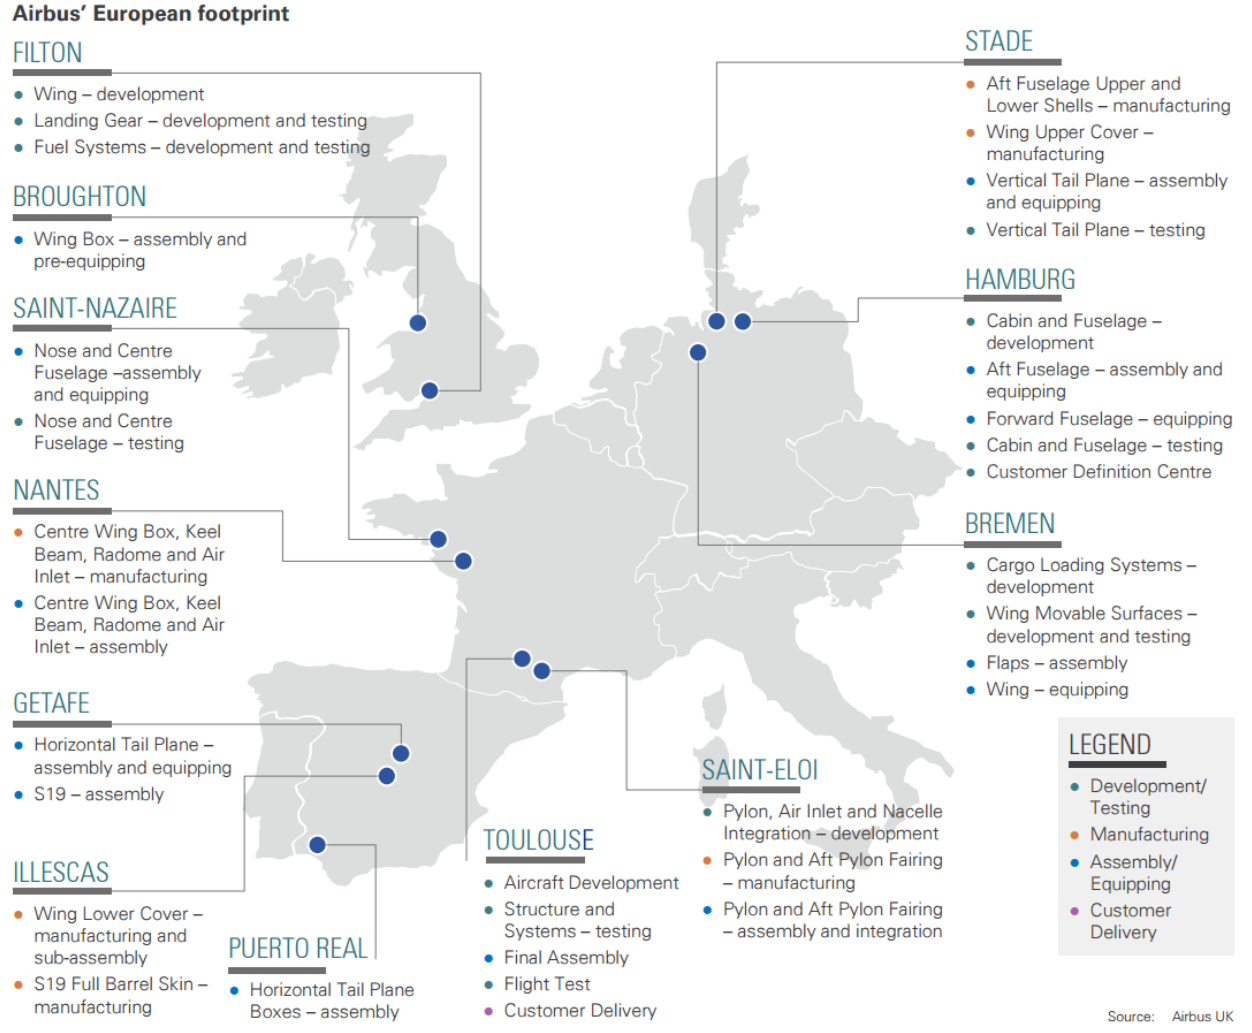
\includegraphics[width=120mm,scale=1]{figs/Airbus-1}
	\caption{Integrated Supply Chains \cite{Airbus:ADS}}
	\label{fig:Airbus} 
\end{figure} 
%\clearpage

Blockchains can offer numerous benefits for streamlining processes and increasing transparency across the supply chain. Coupled with Smart Contracts and IoT, supply chain can become one of the killer applications of the blockchain. Smart Contract platforms such as the Ethereum can use tracking data to automate various functions and events in the supply chain life cycle. Ethereum’s distributed ledger also provides total transparency to all parties involved. By increasing automation within supply chain processes they can reduce complexity and eliminate errors and delays. Some of the key benefit of blockchains in the context of SCM are follows:

\textbf{Transparency:}
Its shared ledger enables all stakeholders to have the same view of the data stored on the blockchain. Transparency is greatly increased due to everyone having real time access to the same data.

\textbf{Traceability and Compliance:}
Every transaction recorded on the blockchain is cryptographically verified. This increases traceability, reduces fraud, and helps to increase compliance for existing products. 

\textbf{Security:}
Any system built on the blockchain is by design highly secure against DDoS attacks and single points of failure. Each transaction on the blockchain is replicated across multiple nodes on a distributed ledger. Each block links to a previous block hence any attacker wanting to modify data in any block will need to modify all subsequent blocks as well.

\textbf{Trust:}
Most traditional Supply Chain Management(SCM) systems allow participants a very limited view throughout the supply chain life cycle. Usually participants only have access to information necessary to successfully realize the next process of the supply chain. This creates information asymmetry between different stake holders. Decentralized blockchain based SCM systems can allow participants to have same view of the entire system and hence reduce information asymmetry and increase trust.
\clearpage
%check motivation again see if i have said that blockchain icnreases trust or allows participants to trust data from untrusted sources, reduces complexity, etc

\subsection{Thesis Objective}
The primary goal of this thesis is to design and develop a secure decentralized supply chain management and shipment tracking system. The backbone for this system will be a Smart Contract for monitoring and regulating supply chain cycles under strict conditions. Two types of decentralized applications will be developed for interacting with the Smart Contract. In order to realize this system following questions and issues must be addressed:

\begin{enumerate}[label=(\alph*)]
\item Which blockchain platform is best suited for development of this system? 
\item How to reduce complexity and increase automation in supply chain processes?
\item Provide real time access to critical information for all relevant stake holders.
\item Enhance the blockchain security model by using Post Quantum Primitives.
\end{enumerate}

The design and requirements of this system are based on a use case scenario presented in chapter \ref{usecase}. 

%check motivation again see if i have said that blockchain icnreases trust or allows participants to trust data from untrusted sources, reduces complexity, etc. Add these as research objectives for our system. I.e. greatly increase trust, provide real time insight into critical data like violation events or some other important event, increase automation. sub questions could be whihc blockchain platform is most useful etc.
%Increase trust in SCM and Information, How to increase trust by using blockchains
